\documentclass[12pt]{article}

\usepackage[a4paper, margin=1in]{geometry}
\usepackage{xcolor}
\usepackage{amsmath}
\usepackage{tcolorbox}
\usepackage{fontawesome5} % icons
\usepackage{hyperref}
\usepackage{graphicx}
\usepackage{float}
\usepackage{comment}
\usepackage[nameinlink,capitalize,noabbrev]{cleveref}
\usepackage{subcaption} % modern replacement for the deprecated subfigure package

\setlength{\parindent}{0pt}

% --- COLOR PALETTE (customize these) ---
\definecolor{maincolor}{HTML}{2A9D8F} % your teal
\definecolor{accentcolor}{HTML}{E76F51}
\definecolor{lightcolor}{HTML}{FFDEAD}

% Tell cleveref how to name your counter
\crefname{exercise}{assignment}{assignments}
\Crefname{exercise}{Assignment}{Assignments}

% --- ASSIGNMENT STYLE ---
\newcounter{exercise}

% Optional label: \exercisetitle[<label>]{<Title>}
\newcommand{\exercisetitle}[2][]{%
  \refstepcounter{exercise}% make this step referenceable/hyperlinked
  \vspace{0.5cm}%
  \colorbox{maincolor}{%
    \makebox[\dimexpr\linewidth-2\fboxsep][l]{%
      \textcolor{white}{\faPen\ Assignment \theexercise:~ #2}%
    }%
  }%
  % If an optional label was provided, set it
  \if\relax\detokenize{#1}\relax\else\label{#1}\fi
  \vspace{0.3cm}%
}


% --- IMPORTANT BOX ---
\newtcolorbox{importantbox}{
  colback=lightcolor,
  colframe=accentcolor,
  arc=4mm,
  boxrule=1pt,
  left=6pt,
  right=6pt,
  top=6pt,
  bottom=6pt
}

% --- PROMPT BOX ---
\newtcolorbox{promptbox}{
  colback=white,
  colframe=maincolor,
  arc=4mm,
  boxrule=1pt,
  left=6pt,
  right=6pt,
  top=6pt,
  bottom=6pt
}

% --- QUESTION BOX (with starred variant and cleveref names) ---
% Requires: \usepackage{hyperref} for \Form/\TextField
%           \usepackage{fontawesome5} for \faEdit

% Cleveref names for the question counter
\crefname{question}{question}{questions}
\Crefname{question}{Question}{Questions}

\makeatletter
\newcounter{question}
\newlength\questionheight
\setlength\questionheight{5cm} % default answer box height

% \question{<text>}                  -> with TextField (default height)
% \question[<height>]{<text>}        -> with TextField (custom height)
% \question*{<text>}                 -> no TextField, still numbered
\newcommand{\question}{\@ifstar{\question@text}{\question@field}}

% Common heading (the calling command increments the counter)
\newcommand{\question@heading}[1]{%
  \vspace{0.3cm}%
  \noindent\textbf{\faEdit\ Question \thequestion: #1}%\\[0.3em]%
}

% Starred form: numbered question without input field
\newcommand{\question@text}[1]{%
  \refstepcounter{question}%
  \question@heading{#1}%
%  \vspace{0.3cm}%
}

% Unstarred form: numbered question with input field (optional height)
\newcommand{\question@field}[2][\questionheight]{%
  \par
  \refstepcounter{question}% keep labels after \question tied to this question
  \noindent
  \begin{minipage}{\linewidth}% keep the question and answer box together
    \question@heading{#2}%
    \\[0.3em]
    \begin{Form}
      \TextField[
        name=Q\thequestion,
        multiline=true,
        width=\linewidth,
        height=#1,
        charsize=10pt,
        bordercolor={0 0 0},
        borderwidth=1.8,
        backgroundcolor={1 1 1}
      ]{}
    \end{Form}
    \vspace{0.3cm}%
  \end{minipage}%
  \par
}
\makeatother

% --- SOLUTION BOX ---
%--- Definition of solution/no solution env to change between the teacher and the student versions --------%

% --- Teacher toggle ---
\newif\ifteacher
\teachertrue% Write teacherfalse for student version and teachertrue for teachers version

% --- Solution environment ---
\newtcolorbox{solutionbox}{colback=gray!10,colframe=black!60!black,arc=1mm,boxrule=1pt}

\ifteacher
\newenvironment{solution}{%
  \begin{solutionbox}\textbf{Solution:}
}{%
  \end{solutionbox}
}
\else
  \excludecomment{solution}
\fi


\begin{document}

\begin{titlepage}

% --- Top spacing ---
\vspace*{1cm}

% --- Project logo ---
\begin{center}
    
\includegraphics[height=3cm]{Figures/Logo_TAI_Transparent.png}
\end{center}

\vspace{0.8cm}

% --- Title page ---
\begin{center}
    {\Huge \bfseries \color{maincolor} Planetary Chemistry: The Quest for Iron Oxide \par}
    \vspace{0.5cm}
    
    {\Large \color{accentcolor} Teaching with AI (TAI) \par}
    
    \vspace{1.5cm}
    
    \begin{center}
{\large
Andrea López Incera$^{2}$, Carme Grimalt Álvaro$^{2}$, Rafael Sánchez Mejías$^{2}$, Mirte van der Eyden$^{1}$  \\[0.3cm]

{\small
$^{1}$ Institut für Fachdidaktik, Universität Innsbruck \\ 
mirte.van-der-eyden@uibk.ac.at \\[0.2cm]


$^{2}$ Departament de didàctica de la matemàtica i les ciències experimentals, Universitat Autònoma de Barcelona \\ 
andrea.lopez.incera@uab.cat
}
}
\end{center}

\end{center}

\vfill

% --- Logos at the bottom ---
\begin{center}
\begin{tabular}{cccc}

\includegraphics[height=1.5cm]{Figures/Logos/universitaet-innsbruck-logo-cmyk-farbe.jpg} &

\includegraphics[height=1.5cm]{Figures/Logos/logotipuab-v1-verd.png} &

\includegraphics[height=1.5cm]{Figures/Logos/EN Co-funded by the EU_POS.jpg} \\

\includegraphics[height=1.5cm]{Figures/Logos/IMG_1189.PNG} &
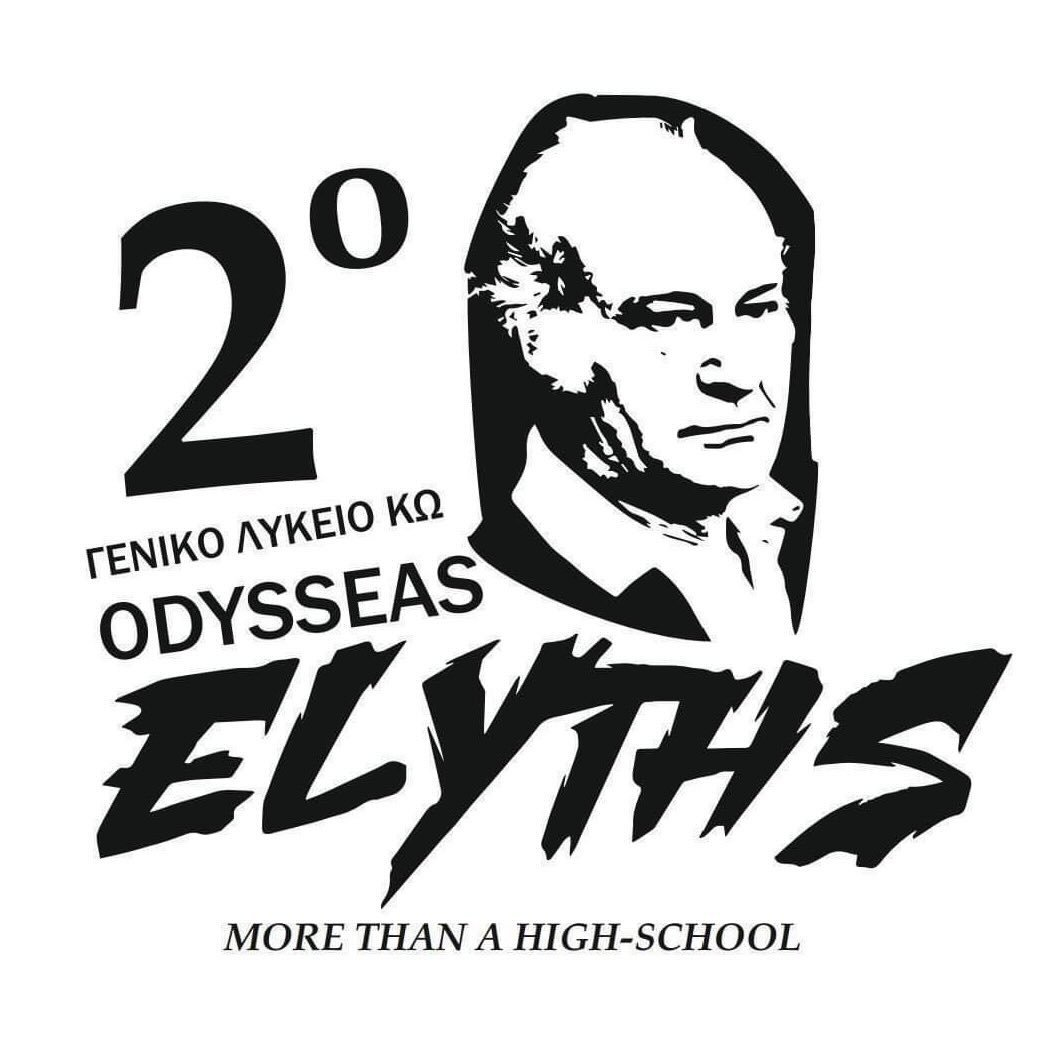
\includegraphics[height=1.8cm] {Figures/Logos/2nd Lyceum of Kos logo.jpg} &

\includegraphics[height=1.5cm]{Figures/Logos/NEXT_prov_logo.png}
\end{tabular}
\end{center}


\vspace{0.5cm}

% Optional footer text
\begin{center}
    {\small Project funded by Erasmus+ Programme of the European Union}
\end{center}

\end{titlepage}

% --- Description of activity ---
\vspace*{0.5\textheight}

Subject: Chemistry


\vspace{0.3cm}

Activity duration: 90 min

\vspace{0.5cm}

Phases:
\begin{enumerate}
    \item Choice and characterization of exoplanet sample with AI-lab (20 min)
    \item Colorimetry in the real lab to get an approximate concentration (30 min)
    \item Filtering and weighing the iron oxide (40 min)
\end{enumerate}

Learning goals:

\begin{itemize}
    \item Learn about the characterization of substances with an AI lab that can perform fast, small experiments embedded in the exoplanet context.
\item Analytical chemistry: learn how to do a colorimetry to estimate a concentration.
\item Learn techniques such as filtering or dehydration 
\item Work with stoichiometric relations of chemistry reactions and compute masses and solution concentrations


\end{itemize}

\newpage

% --- HEADER / BRANDING ---
\begin{center}
    {\LARGE \color{maincolor} Planetary Chemistry: The Quest for Iron Oxide}\\[5pt]
    {\large \textit{A chemistry lesson with AI}}\\
    \rule{\linewidth}{1pt}
\end{center}

\vspace{0.5cm}

\begin{importantbox}
\textbf{Challenge}: The Aurora Network is a system of scientific stations spread across several exoplanets that monitor climate, geology, and possible signs of life. After a powerful radiation storm damaged one station, engineers need to manufacture new \textbf{iron-oxide-rich} ceramic bricks to restore the protective shielding around sensitive instruments. Because transporting construction materials from Earth is slow and costly, scientists are searching for a local source of iron at the exoplanets. Your mission is to use a rover and its AI laboratory to identify the planet most likely to contain iron-rich compounds and determine which sample could produce the greatest amount of iron oxide (\(\mathrm{Fe_2O_3}\)). The results of your laboratory analysis will help decide whether the deposit can provide enough material to repair the station's shielding.
\end{importantbox}




\vspace{0.3cm}


% --- Assignment ---
\exercisetitle{Send a sample to Earth}

You can control an AI-embedded lab inside the rover that is exploring your assigned exoplanet. The rover should take a sample and send it to Earth for further analysis. Your goals in this assignment are:

\begin{itemize}
  \item Choose which site to take a sample from.
  \item Identify which is the most likely substance in the sample.
\end{itemize}

\textcolor{maincolor}{\textbf{\faPen\ Go to the link provided by the teacher that will take you directly to the AI-lab of your corresponding rover.}} How to use it:
\begin{itemize}
  \item The rover has a maximum energy of 100 points. Going to a site costs 3 points. Doing an experiment costs 10 points. Once the rover is out of energy, you won't be able to do anything else.

  \item Once you have moved the rover to a site, you can choose experiments in the dropdown menu. The AI will then give you the result of the chosen experiment for a sample taken from that site.

  \item You can chat with the AI for free in the Chat log, so don't hesitate in asking as many questions as you want.

\end{itemize}

\vspace{0.5cm}
\textcolor{accentcolor}{\textbf{\faLightbulb\ Initial ideas}}

\question{Look at the overview image with all the sites. Which ones do you think can contain an iron compound and why?}



\vspace{0.5cm}
\textcolor{accentcolor}{\textbf{\faLightbulb\ Constructing new ideas}}

\question*{In the box below, write the conclusions you get after interacting with the AI lab on each of the sites:}

\vspace{0.3cm}
\begin{Form}

\renewcommand{\arraystretch}{1.8}

\begin{tabular}{|p{1.5cm}|p{3cm}|p{10cm}|}
\hline
\textbf{Site} & \textbf{Compound} &  \textbf{Why? Conclusions from experimental results} \\
\hline

\TextField[name=site1,width=\linewidth,height=1cm,multiline=true,bordercolor={0 0 0}]{} &
\TextField[name=compound1,width=\linewidth,height=1cm,multiline=true,bordercolor={0 0 0}]{} &
\TextField[name=conclusions1,width=\linewidth,height=1cm,multiline=true,bordercolor={0 0 0}]{} \\
\hline

\TextField[name=site2,width=\linewidth,height=1cm,multiline=true,bordercolor={0 0 0}]{} &
\TextField[name=compound2,width=\linewidth,height=1cm,multiline=true,bordercolor={0 0 0}]{} &
\TextField[name=conclusions2,width=\linewidth,height=1cm,multiline=true,bordercolor={0 0 0}]{} \\
\hline

\TextField[name=site3,width=\linewidth,height=1cm,multiline=true,bordercolor={0 0 0}]{} &
\TextField[name=compound3,width=\linewidth,height=1cm,multiline=true,bordercolor={0 0 0}]{} &
\TextField[name=conclusions3,width=\linewidth,height=1cm,multiline=true,bordercolor={0 0 0}]{} \\
\hline

\TextField[name=site4,width=\linewidth,height=1cm,multiline=true,bordercolor={0 0 0}]{} &
\TextField[name=compound4,width=\linewidth,height=1cm,multiline=true,bordercolor={0 0 0}]{} &
\TextField[name=conclusions4,width=\linewidth,height=1cm,multiline=true,bordercolor={0 0 0}]{} \\
\hline

\end{tabular}
\end{Form}

\begin{solution}
For each exoplanet, look into its corresponding dossier to get the answers to this question (\url{https://scientificailab.streamlit.app/RoverLab}, then go to the dropdown menu "Full scenario details". Never share this webpage with the students! The students should get their own link.). In the dossier, there is a detailed explanation of each site, which substance it contains, and how the substance reacts to each of the experiments. See the additional "Teacher Guide" for more details.
\end{solution}


\question{Which site have you finally chosen to get a sample and send it to Earth? Which substance do you think it contains?} 

\begin{solution}
They should choose Site 1 (for all exoplanets). What they get there is an Iron (III) chloride solution with different concentration for each exoplanet. Some planets have here a decoy solution (it seems it is Iron (III) chloride but it is not). Students only know about this when they do the reaction with the KOH.
\end{solution}

\vspace{1cm}

% --- Assignment  ---

\exercisetitle{Analyzing the sample's concentration at the Earth's lab}

The sample has arrived at the Earth's lab. Here, you will have to further analyze it to later conclude which exoplanet has the largest potential to get the biggest amount of iron oxide. Your goal now is:

\begin{itemize}
  \item Do a colorimetry to estimate the sample concentration.
\end{itemize}

\vspace{0.5cm}
\textcolor{accentcolor}{\textbf{\faLightbulb\ Initial ideas}}

\question{Ask the AI (or look for information elsewhere on the internet) about the possible ways that one can get $\mathrm{Fe_2O_3}$ from the substance of the sample you sent to Earth. Write all the steps of the process here, including the chemical reactions (properly balanced!). Note that you need to do these steps with substances that are available at your lab.}\label{q:steps_reactions}

\begin{solution}
See Teachers Guide for details and for the properly balanced reactions. In summary:
\begin{enumerate}
  \item Make $FeCl_3$ react with $KOH$ to get $Fe(OH)_3$ (precipitated).
  \item Filtrate the precipitated $Fe(OH)_3$.
  \item Thermally decompose the hydroxide $Fe(OH)_3$ into an oxide $Fe_2O_3$
\end{enumerate}

\end{solution}

\question{Why do you need to estimate the sample concentration before doing anything else?}

\begin{solution}
  To know how much $KOH$ to add in order to get all the Iron(III) chloride to react (in turn, to extract as much iron oxide as possible from the sample).
\end{solution}

\question{How would you estimate the concentration (in moles of solute/L of solution) of the sample solution you got (considering that you cannot distil the water out)?}

\begin{solution}
  Getting to the idea of colorimetry. Before the next step, students should understand how the colorimetry works.
\end{solution}

\vspace{0.5cm}
\textcolor{accentcolor}{\textbf{\faLightbulb\ Constructing new ideas}}

\textcolor{maincolor}{\textbf{\faPen\ Do the colorimetry of the sample to get its estimated concentration.}} To do that, first, you need to create several control samples of which you know the concentration, to then compare the color of the exoplanet sample to the color of the control samples and estimate its concentration. 

\question{Make a list of the concentrations you created for the control samples.}

\question{Which is your best estimation of the exoplanet's sample concentration based on the colorimetry?}


% --- Assignment  ---

\exercisetitle{Getting the iron (III) oxide and measuring its mass}

As you have seen, doing the colorimetry is not a very precise measurement for how much iron is in the sample. But we need this initial measurement for our next step. We now are going to extract the iron oxide and measure it. Your goals now are:

\begin{itemize}
\item Do the chemical reactions needed to get the iron oxide $\mathrm{Fe_2 O_3}$.
  \item Measure the final mass of iron oxide you get from the sample.
\end{itemize}

\question{Look again at the answer of Question~\ref{q:steps_reactions}. How much $KOH$ do you need to add to your exoplanet sample to make sure that *all* the $Fe(Cl)_3$ precipitates? Write the calculations here.}

\textcolor{maincolor}{\textbf{\faPen Look again at the answer of Question~\ref{q:steps_reactions} for the steps and chemical reactions you are about to do.
\begin{itemize}
  \item  Do the reaction with the $KOH$. 
\item Afterwards, filter the precipitated substance and heat it up.
\item Weigh the resulting substance. 
\end{itemize}
}}

\question{Describe the resulting substance. Is it what you expected to get in terms of color, consistency, etc. (you can check with an AI what is the expected aspect of the $Fe_2O_3$)? If not, what do you think has happened?}

\begin{solution}
See Teachers Guide.
\end{solution}

\question{Compute the mass of $Fe_2O_3$ you expected to get if the concentration of the sample was the one you estimated with the colorimetry. Is the one you actually got larger or smaller?}

\begin{solution}
See Teachers Guide for the expected masses for each of the samples.
\end{solution}


\vspace{0.5cm}
\textcolor{accentcolor}{\textbf{\faLightbulb\ Closing the challenge}}

\vspace{0.3cm}
\textcolor{maincolor}{\textbf{\faPen\ Write in your exoplanet file the resulting final weight of the iron oxide.}}

\vspace{0.5cm}
\textcolor{accentcolor}{\textbf{\faLightbulb\ What have we learned?}}

\vspace{0.3cm}
\textcolor{maincolor}{\textbf{\faPen\  Write in your file the things you have learned in this lesson (Reflections) and how you used AI for science in this lesson (AI assistance).}}



\end{document}
